% D06-004. PDR-05, §11, таблицы 13--15, рисунок 13.
\section{Проверка РНМ на программе испытательных режимов БАВР}
\label{sec:ch5_rtds_validation}
\conceptsource{Статья 5, раздел 11. Режимы двигательной нагрузки,
100 опытов и две секции, формульные и нейросетевые варианты,
условные ошибки и устойчивое воспроизведение переходов.
Ниже используется завершённый снимок от 20.09.2026,
а не незавершённый третий просмотр авторской разметки.
Числа предварительны относительно продолжающегося пересмотра
эталона. Методика доступна для вычитки; окончательная приёмка
результатов требует авторской проверки указанных режимов.}

\subsection{Назначение и физическое содержание программы}
\conceptsource{Статья 5, подразделы 11.1--11.2.
Программа описывается как основание конкретного опыта,
без нового утверждения нормативной обязательности.
Первичный отраслевой документ требует отдельной приёмки.}

Эксплуатационный архив содержит разнообразные процессы,
но состав записей зависит от практики регистрации
и последующего отбора сложных случаев.
Для дополнительной проверки использован другой набор,
сформированный по программе испытательных режимов БАВР.
Проверяется поведение измерительного органа
на заранее заданных нарушениях электроснабжения
и состояниях двигательной нагрузки.

В модели электроснабжения нефтеперекачивающей станции
представлены внешняя сеть 110~кВ,
трансформаторы, распределительные устройства 6~кВ,
линии, реакторы, синхронные и асинхронные двигатели.
Для синхронных машин учитываются возбуждение
и его регулирование, для механической нагрузки
насосная моментно-скоростная характеристика.
После нарушения питания вращающиеся машины
могут поддерживать остаточное напряжение шин
и изменять направление перетока мощности.
Поэтому одного уровня напряжения недостаточно
для описания требуемой реакции РНМ.

Программа включает отключения воздушных линий,
короткие замыкания разного вида, места и длительности,
изменения схемы и состава работающих агрегатов.
Повреждения внешней сети и внутренние повреждения шин
создают разные условия действия автоматики.
В первом случае важно своевременно подготовить
восстановление питания, во втором сохранить запрет
на включение резерва на повреждённую секцию.
Отдельного рассмотрения требуют ненагруженные вводы
и состояние после размыкания выключателя.
Отсутствующий ток не даёт надёжно наблюдаемого направления.

Использованы 100 осциллограмм с обозначениями опытов программы.
Каждая содержит две секции.
На вход органа подаются ток соответствующего ввода
и напряжение его сборных шин.
После отключения вводного выключателя именно напряжение шин
характеризует остающуюся двигательную нагрузку.
Напряжение со стороны отключённого источника
относится к другому электрическому узлу.

Ниже приведены результаты для зафиксированной версии
экспертных меток. Их физический пересмотр продолжается,
поэтому численные выводы являются предварительными.
Исследование характеризует измерительный орган
по зарегистрированным сигналам.
Испытание всей логики БАВР с выключателями,
блокировками и полным временем переключения
остаётся отдельной задачей.

% D06-005 R5-09 BEGIN
\ifdefined\AuthorReview
\par\smallskip\begingroup\small\raggedright\color{red!60!black}
\noindent\textbf{Примечание рецензента [R5-09], согласовать целевое состояние.} Выше сказано, что отсутствующий ток не даёт надёжно наблюдаемого направления. В 5.2 подпороговый ток при достаточной поляризации, однако, является применимым нулевым выходом, то есть отсутствием блокировки. Физическая неопределённость знака потока и целевое состояние органа здесь должны различаться столь же явно. Уточнить, какое правило использовано для разгруженного ввода и после отключения выключателя. Это вопрос к единству эталона, а не предложение автоматически изменить метки RTDS.\par\endgroup\smallskip
\fi
% D06-005 R5-09 END

\subsection{Единицы оценки и состав сравнения}
\conceptsource{Статья 5, подраздел 11.3.
25 вариантов, усреднение по опыту и секции,
доли экспертных состояний и начальная неготовность.}

На одинаковых сигналах проверяются девять формульных органов
и 16 наборов нейросетевых весов.
Для каждой из четырёх сетей сохранены последние
и выбранные по прежней валидации состояния
до и после экспертного этапа.
До него выбор опирался на автоматические цели,
после него на ручную разметку.
Всего сопоставляются 25 вариантов измерительного органа.
Записи RTDS не использовались для обучения этих весов
или выбора соответствующих эпох.
Однако H123-D24 предложена после просмотра
результатов прежних моделей на этой программе.
Для неё набор является повторно используемым диагностическим
материалом и не считается полностью новым испытанием
архитектурного предположения.

Каждая запись содержит 64\,000 отсчётов
с частотой регистрации 20~кГц и длительностью 3,2~с.
Две секции дают 200 пар опыт--секция
и 12,8~млн отсчётов полного состояния.
Соседние отсчёты принадлежат одному процессу,
а секции одного опыта электрически связаны.
Поэтому эти числа не означают миллионы независимых испытаний.

Сначала показатель вычисляется для каждой пары опыт--секция,
затем пары усредняются с равными весами.
При групповой оценке неопределённости секции
объединяются внутри исходного опыта.
Основной показатель учитывает полное состояние.
Рядом определяется точность направления
при совместной применимости эксперта и органа
и покрытие экспертно применимого времени.
Так уменьшение числа ответов не может незаметно
повысить оценку направления.
Начальное накопление измерений остаётся в основной оценке.
Как и в плотной экспертной проверке,
здесь используется ранний пуск после первого
полнопериодного преобразования Фурье.
Эта начальная доступность ответа отличается
от накопления полного десятипериодного входного контекста
с его дополнительной спектральной предысторией.

В экспертных метках прямое направление занимает 76,52\%
отсчётов, обратное 23,23\%, неприменимость 0,25\%.
Доля обратного направления на первой секции равна 34,00\%,
на второй 12,45\%.
Постоянный применимый ответ о прямом направлении
дал бы 76,52\% совпадений полного состояния.
Общая точность поэтому рассматривается вместе
с обнаружением менее частого обратного направления
и с правильным отказом от решения.

% D06-005 R5-10 BEGIN
\ifdefined\AuthorReview
\par\smallskip\begingroup\small\raggedright\color{red!60!black}
\noindent\textbf{Примечание рецензента [R5-10], инженерная наглядность.} Для электроэнергетика нужна компактная схема двух секций с местами измерения токов и шинных напряжений и краткая группировка 100 опытов. Сейчас электрическая модель и различие внешнего/внутреннего повреждения описаны только словами. Использовать существующую схему и программу, сохранив источник и авторство; не придумывать параметры сети или новые опыты. Полную таблицу вариантов можно вынести в приложение. Это особенно поможет объяснить единственный опыт с разгруженной секцией.\par\endgroup\smallskip
\fi
% D06-005 R5-10 END

\subsection{Сопоставление формульных органов}
\conceptsource{Статья 5, таблица 13 и разгруженная секция.
Результат этой программы не заменяет экспертный архив сложных случаев.}

Результаты формульных реализаций приведены
в таблице~\ref{tab:ch5_rtds_analytical}.
Точность направления относится только к совместно применимым
отсчётам, покрытие к экспертно применимым,
полное состояние ко всей проверяемой сетке.
Последний столбец показывает пары,
где есть непрерывное расхождение длиннее 20~мс.

\begin{table}[htbp]
\centering\small
\caption{Формульные органы на 100 испытательных режимах}
\label{tab:ch5_rtds_analytical}
\setlength{\tabcolsep}{3pt}
\begin{tabular}{p{0.35\textwidth}rrrr}
\toprule
Орган & \shortstack{Точность\\направления, \%}
 & \shortstack{Покрытие,\\\%}
 & \shortstack{Верное\\состояние, \%}
 & \shortstack{Пар с ошибкой\\$>20$~мс, из 200} \\
\midrule
Фазный угловой & 98,04 & 98,94 & 96,77 & 43 \\
Угловой прямой последовательности & 97,53 & 98,94 & 96,25 & 57 \\
Фазный мощностной & 97,04 & 98,94 & 95,80 & 64 \\
Мощностной прямой последовательности & 96,92 & 98,94 & 95,65 & 64 \\
Адаптивный & 96,95 & 99,01 & 95,75 & 83 \\
Двухвыборочный & 96,46 & 98,91 & 95,15 & 39 \\
Пятивыборочный & 92,18 & 99,00 & 91,05 & 70 \\
БМРЗ, реактивно-токовая ветвь & 96,49 & 98,94 & 95,26 & 103 \\
Адаптация БАВР-072 & 97,11 & 99,01 & 95,89 & 72 \\
\bottomrule
\end{tabular}
\end{table}

Наибольшее среднее совпадение полного состояния
среди формульных органов здесь имеет фазная угловая реализация.
Это отличается от сравнения на специально отобранных
сложных эксплуатационных записях.
Изменился состав режимов,
а не исчезли ограничения пофазной характеристики.
В единственном опыте с разгруженной секцией
среднее совпадение фазного углового органа по двум секциям
составляет 74,15\%, адаптивного 99,29\%.
Такой режим представлен одним опытом
и слабо влияет на общий средний показатель,
хотя важен для предметной проверки БАВР.

\subsection{Изменение нейросетевого решения после экспертного этапа}
\conceptsource{Статья 5, таблица 14, раздельные последние
и ранее выбранные веса. RTDS не используется для нового выбора эпохи.}

Для сетей в таблице~\ref{tab:ch5_rtds_neural}
различены последние и ранее выбранные веса.
В двух последних столбцах используются только последние.
Точность направления вновь относится
к совместной применимости с экспертом.

\begin{table}[htbp]
\centering\small
\caption{Нейросетевые органы до и после экспертной адаптации на RTDS}
\label{tab:ch5_rtds_neural}
\setlength{\tabcolsep}{3pt}
\begin{tabular}{p{0.20\textwidth}p{0.135\textwidth}rrrr}
\toprule
Вход & Этап & \shortstack{Верное\\состояние, \%\\последние}
 & \shortstack{То же, \%\\выбранные}
 & \shortstack{Точность\\направления, \%}
 & \shortstack{Пар с ошибкой\\$>20$~мс, из 200} \\
\midrule
Два среза & Учитель & 95,90 & 96,64 & 96,74 & 72 \\
Два среза & Эксперт & 96,38 & 96,34 & 97,22 & 63 \\
Пять срезов & Учитель & 95,92 & 96,12 & 96,75 & 71 \\
Пять срезов & Эксперт & 96,26 & 96,07 & 97,10 & 62 \\
Последова\-тельность & Учитель & 95,11 & 95,15 & 95,94 & 89 \\
Последова\-тельность & Эксперт & 96,29 & 95,70 & 97,13 & 87 \\
H123-D24 & Учитель & 95,17 & 95,08 & 96,01 & 83 \\
H123-D24 & Эксперт & 96,16 & 95,91 & 97,00 & 77 \\
\bottomrule
\end{tabular}
\end{table}

При сравнении последних эпох экспертный этап
увеличивает среднее совпадение состояния на 0,48 пункта
для двух срезов, 0,34 для пяти,
1,18 для последовательности и 0,99 для H123-D24.
Но улучшение не распространяется на каждый опыт.
У H123-D24 результат выше в 124 парах,
ниже в 64 и не меняется в 12.
Следовательно, средний прирост не заменяет
адресной проверки ухудшившихся режимов.

Выбор эпохи по исходной валидации
не обеспечивает наибольшего результата на новой программе.
Два среза до экспертного этапа имеют 96,64\%
для ранее выбранных весов, что выше результата
последней эпохи и дообученного варианта.
У H123-D24, напротив, последние экспертные веса
дают 96,16\% против 95,91\% у выбранных.
Повторно выбирать веса по этой таблице
и затем считать ту же программу независимой проверкой нельзя.

Для последних экспертных сетей совпадение полного состояния
первой и второй секций составляет соответственно
96,04 и 96,72\% для двух срезов,
95,83 и 96,68\% для пяти,
95,99 и 96,58\% для последовательности,
95,94 и 96,38\% для H123-D24.
При объединении применимых отсчётов H123-D24
правильно воспроизводит 92,74\% обратного направления
и 97,51\% прямого с учётом отказов.
Компактная модель пяти срезов имеет 91,24 и 98,09\%.
Улучшение одного направления сочетается
с ухудшением другого и не сводится к общему превосходству.

\subsection{Неприменимость и контроль измерительных сигналов}
\conceptsource{Статья 5, подразделы 11.3, 11.5--11.6.
Редкий отрицательный класс и отдельные сомнительные пики
не превращены в подтверждённую диагностику качества напряжения.}

В зафиксированном эталоне неприменимые участки
выделены в обеих секциях трёх опытов.
Они содержат 31\,982 отсчёта,
что соответствует 1,5991~с суммарного секционного времени.
Все 25 вариантов органов пропускают
это экспертно неприменимое время.
Следовательно, ограничение относится
как к сетям, так и к формульным реализациям.

При этом среднее совпадение применимости у сетей
составляет 99,13\%, а покрытие экспертно применимых
отсчётов 99,37\%.
Высокая общая доля соседствует
с отсутствием обнаруженных участков редкого отрицательного класса.
Первые 399 отсчётов, необходимые для начального Фурье,
сети не выдают направление, а далее определяют его.
Эта начальная неготовность не доказывает
способности распознавать неприменимый режим
после начала работы.

Поддержка отрицательного класса ограничена тремя опытами,
их экспертное рассмотрение продолжается.
Результат указывает на несовпадение критериев применимости
и необходимость адресного разбора.
Он не оценивает вероятность пропуска
такого состояния в эксплуатации.

Отдельно контролируется правдоподобие входных сигналов.
В восьми из 200 секционных записей
максимальный модуль мгновенного фазного напряжения
превышает удвоенную номинальную фазную амплитуду.
Наибольший зарегистрированный пик составляет 128,44~кВ,
или 26,22 номинальной фазной амплитуды сети 6~кВ.
Здесь сравниваются мгновенные пики,
а не действующие значения напряжения.

Такой выброс требует проверки модели энергосистемы,
способа регистрации и связи с коммутацией.
Его нельзя автоматически считать установленным
физическим перенапряжением или молча исправлять.
Записи сохранены в текущем сравнении.
Вывод о диагностике аномального напряжения
отложен до физического разбора сигналов
и уточнения соответствующего экспертного эталона.

\subsection{Ошибочное время и неустойчивость решения}
\conceptsource{Статья 5, таблица 15, раздельные определения
смен направления и переключений вне переходных зон.}

Совпадение H123-D24 с экспертом на уровне 96,16\%
соответствует примерно 38,37~мс ошибочного состояния
на секунду записи.
В таблице~\ref{tab:ch5_rtds_engineering}
общая ошибка дополнена условными ошибками направления,
длительными расхождениями и неустойчивостью.
Две секции здесь объединены внутри опыта.
Поэтому число опытов с длительной ошибкой
отличается от числа секционных пар
в предшествующих таблицах.

\begin{table}[htbp]
\centering\small
\caption{Инженерные показатели на 100 опытах RTDS}
\label{tab:ch5_rtds_engineering}
\setlength{\tabcolsep}{3pt}
\begin{tabular}{p{0.28\textwidth}rrrrr}
\toprule
Орган & \shortstack{Ошибка,\\мс/с}
 & \shortstack{Ложное\\прямое, \%}
 & \shortstack{Ложное\\обратное, \%}
 & \shortstack{Опытов\\$>20$/$>100$~мс}
 & Переключений \\
\midrule
Фазный угловой & 32,28 & 4,99 & 0,84 & 35/15 & 592 \\
Адаптивный & 42,54 & 14,57 & 0,76 & 58/36 & 853 \\
Сеть, два среза & 36,21 & 11,99 & 0,75 & 39/24 & 3870 \\
Сеть, пять срезов & 37,45 & 12,71 & 0,89 & 40/25 & 4049 \\
Сеть, последовательность & 37,11 & 13,12 & 0,72 & 63/27 & 4014 \\
Сеть H123-D24 & 38,37 & 10,07 & 1,34 & 53/26 & 3480 \\
\bottomrule
\end{tabular}
\end{table}

Ложное прямое отнесено ко времени экспертного обратного,
ложное обратное ко времени прямого.
Последний столбец учитывает переключения полного состояния
вне начального накопления и ближайших зон экспертных переходов.
Выходная выдержка или гистерезис при таком подсчёте
в орган не добавляются.
Речь идёт об анализе его непосредственного ответа.
\figurereview{Два значения таблицы уточнены по неизменной
первичной сводке. Ложное прямое фазного углового органа
равно 4,99474\%, что округляется до 4,99\%,
ложное обратное H123-D24 равно 1,34479\%, до 1,34\%.
В статье указаны 5,00 и 1,35\%. Остальные перенесённые
ячейки совпали с сохранёнными отчётами.
Исходная статья не изменялась.}

По общему ошибочному времени H123-D24
лучше адаптивного органа на 0,42 процентного пункта,
но парный 95\%-й интервал разности
простирается от $-1{,}16$ до $+0{,}21$ пункта.
Он включает отсутствие преимущества.
При этом ложное прямое H123-D24 занимает 10,07\%
экспертного времени обратного,
а ложное обратное 1,34\% времени прямого.
Обратное направление присутствует в 97 опытах,
прямое во всех 100.
Средняя доля ошибок скрыла бы эту асимметрию.

Отдельный подсчёт смен направления
даёт 173 перехода в экспертном эталоне,
959 у адаптивного органа и 665 у фазного углового.
У последних экспертных сетей получены
4032 перехода для двух срезов,
4188 для пяти и 4209 для последовательности.
У H123-D24 их 3600,
на 588, или 14,0\%, меньше,
чем у компактной модели пяти срезов.
Но пар с ошибкой длиннее 20~мс
у неё больше, 77 вместо 62.

Этот подсчёт отличается от последнего столбца
таблицы~\ref{tab:ch5_rtds_engineering}.
Смена направления требует применимости
на двух соседних отсчётах и не исключает
все области экспертного перехода.
Поэтому числа 3600 и 3480 относятся к разным событиям.
Их нельзя использовать как два измерения
одной и той же частоты дребезга.

У H123-D24 до экспертного этапа было
2825 смен направления, после него 3600.
Среднее согласие улучшилось,
но число переключений увеличилось на 775.
Уменьшение спектра и увеличение глубины
тем самым не устранили неустойчивость.
Дополнительное подтверждение выхода
может изменить её, но одновременно добавит задержку.
Такое изменение требует самостоятельного опыта.

Порог 20~мс в таблицах служит описательной границей
одного периода сети, а не установленным допуском БАВР.
Часто переключающийся орган может разбить
длительное расхождение на несколько коротких.
Поэтому число эпизодов рассматривается вместе
с суммарным временем ошибки и переключениями.
Ни одна из этих величин сама по себе
не равна числу ошибочных команд выключателю.

% D06-005 R5-11 BEGIN
\ifdefined\AuthorReview
\par\smallskip\begingroup\small\raggedright\color{red!60!black}
\noindent\textbf{Примечание рецензента [R5-11], границы быстродействия.} Временные показатели описывают положение ответа на записанной осциллограмме. Для перехода к работающему РНМ ещё нужны период обновления, время формирования признаков и расчёта сети на выбранном устройстве, а также задержка выдачи результата. Наличие ответа на каждом отсчёте плотной сетки не доказывает возможность такого темпа вычислений. Особенно это относится к H123-D24. Достаточно зафиксировать отсутствующий этап проверки; не переносить сюда времена CPU другой серии из главы 4. Удержание 5 мс в анализе также не является измеренным временем реализации выходной логики.\par\endgroup\smallskip
\fi
% D06-005 R5-11 END

\subsection{Устойчивое воспроизведение смены направления}
\conceptsource{Статья 5, подраздел 11.6 и рисунок 13.
Взаимно однозначное сопоставление, удержание 5 мс,
различные знаменатели двух типов перехода.}

Реакция на экспертный переход проверяется
по правилам раздела~\ref{sec:ch5_engineering_verification}.
Для окна сопоставления $\pm100$~мс
определяется доля достаточно наблюдаемых переходов,
на которые получен ответ не позднее заданного срока.
Новое состояние должно сохраняться не менее 5~мс.
Опережающий ответ учитывается,
если он сохраняется после экспертной границы.
Пропуски остаются в знаменателе.

Из 49 экспертных переходов к прямому направлению
16 имеют новое состояние короче 5~мс.
Из 124 переходов к обратному такой случай один.
Поэтому при сроке 20~мс в сравнении участвуют
33 и 123 перехода соответственно.
Исключённые короткие состояния сохраняются
в полном ошибочном времени
и требуют отдельного физического рассмотрения.

Результат показан на рисунке~\ref{fig:ch5_rtds_event_response}.
H123-D24 своевременно воспроизводит
122 из 123 переходов к обратному направлению.
Модель пяти срезов и адаптивный орган воспроизводят
по 118, фазный угловой 120.
Для перехода к прямому направлению
получены соответственно 23, 11, 13 и 30
ответов из 33.
Различие двух направлений не видно
по одной медиане задержки найденных ответов.

\begin{figure}[p]
\centering
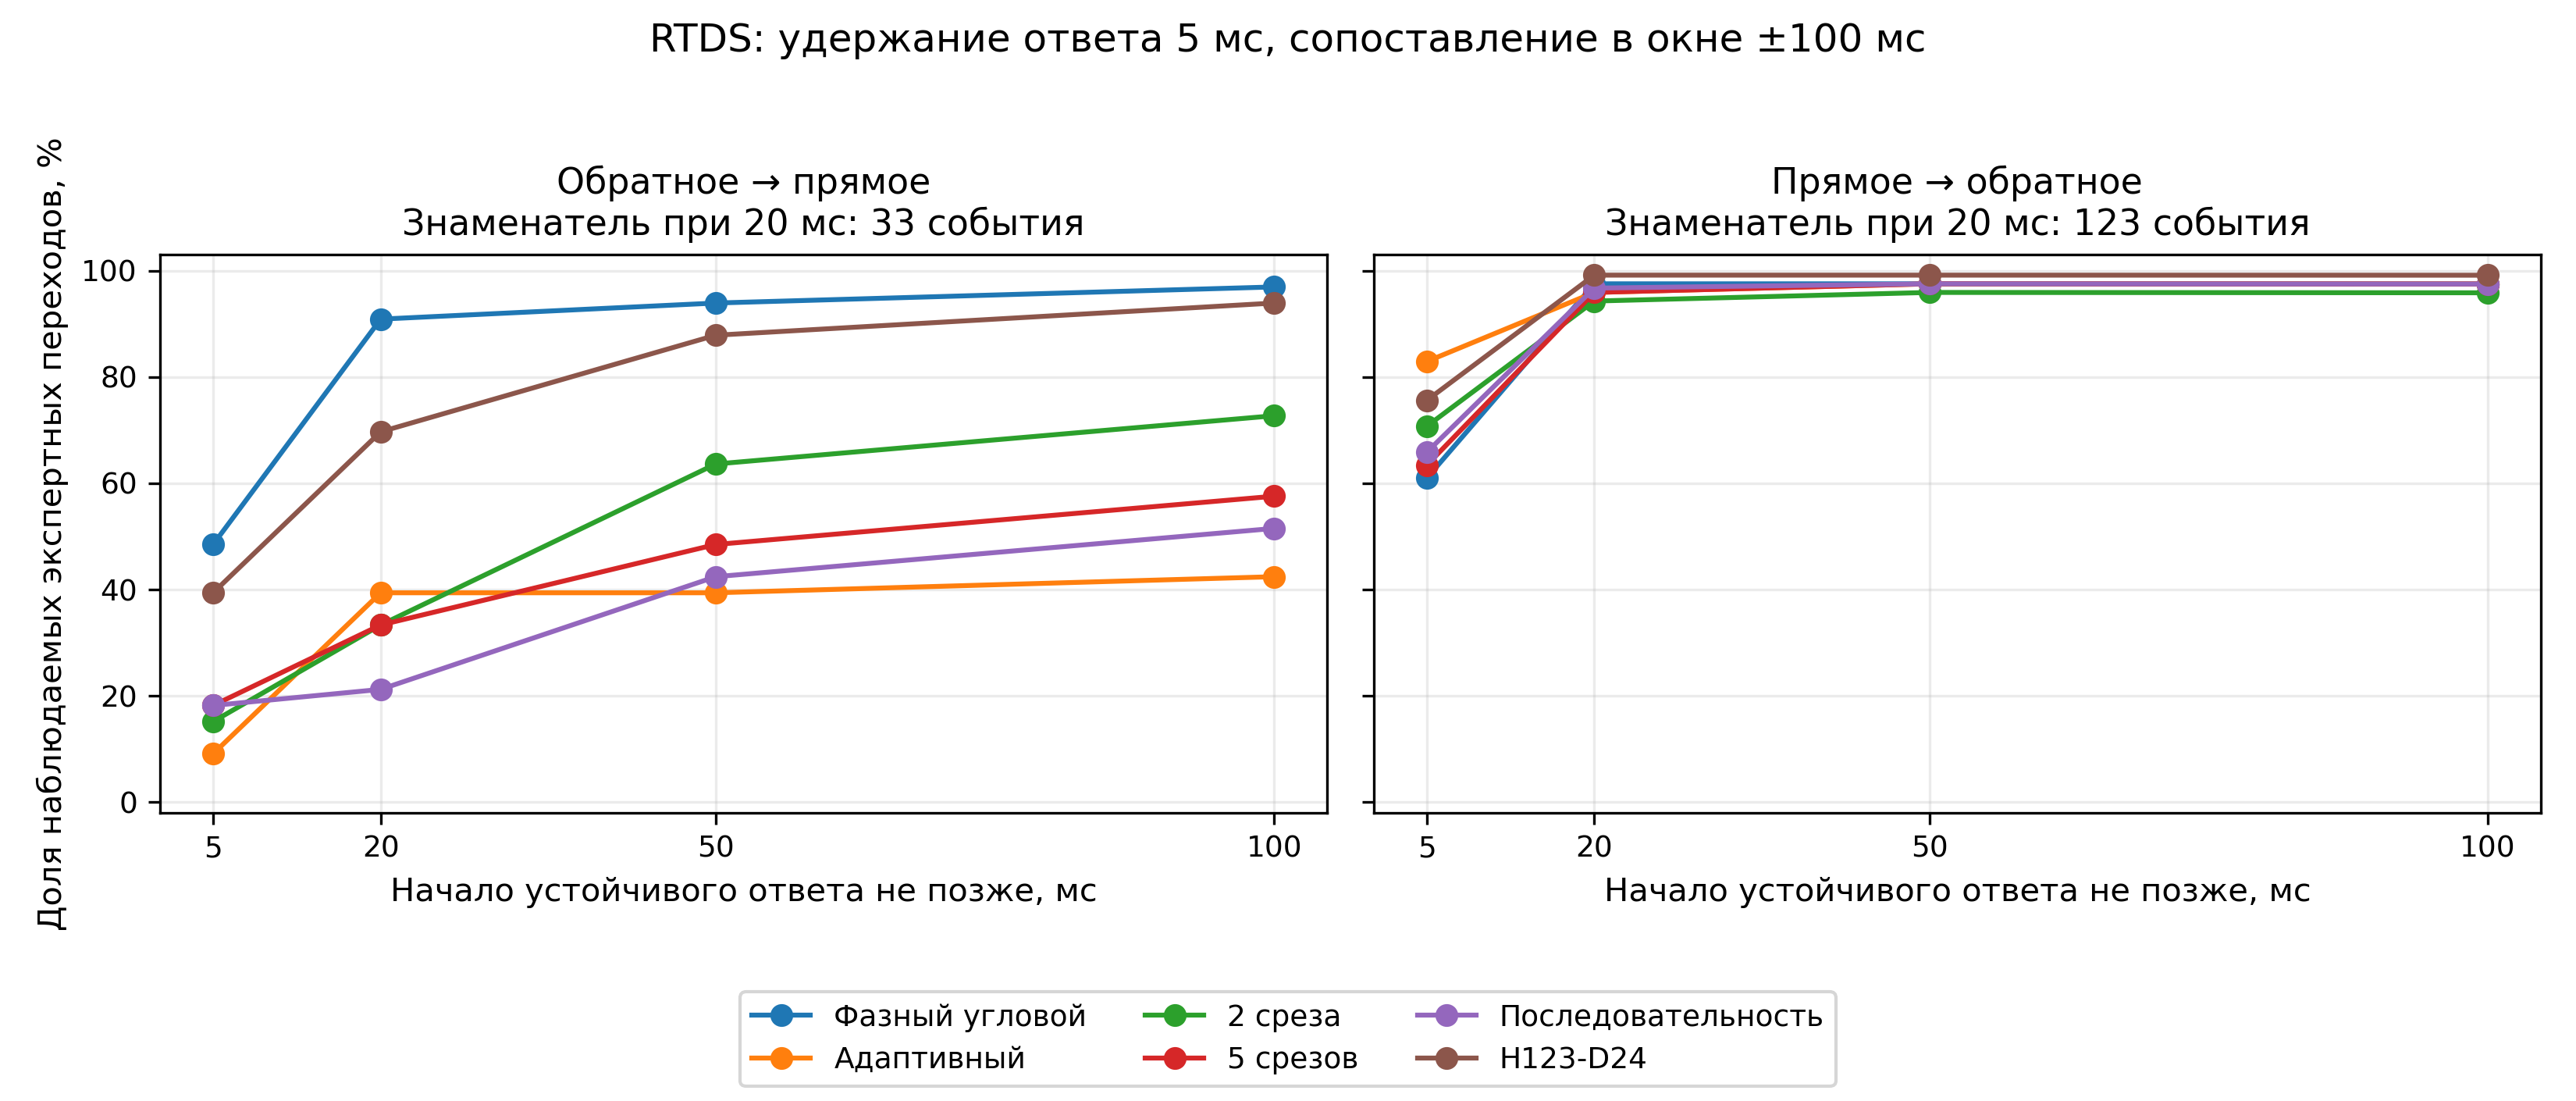
\includegraphics[width=\textwidth]{figures/ch05/ch05_rtds_event_response_article.png}
\caption{Доля своевременно начавшихся и удержанных
не менее 5~мс ответов на экспертную смену направления.
Сопоставление в окне $\pm100$~мс,
пропуски включены в знаменатель}
\label{fig:ch5_rtds_event_response}
\figurereview{Исходный рисунок 13 статьи 5.
Числа относятся к завершённому снимку инженерного аудита.
После завершения авторской перепроверки RTDS
обновить этот рисунок и таблицы по одному эталону.
Для печати увеличить подписи, не менять знаменатели
и не называть горизонтальную ось временем выключателя.}
\end{figure}

Дополнительное исключение экспертной границы
и следующих 5~мс повышает совпадение
полного состояния лишь незначительно.
У фазного углового органа оно меняется
с 96,77 до 96,87\%, у адаптивного с 95,75 до 95,82\%,
у экспертной модели двух срезов с 96,38 до 96,45\%,
у H123-D24 с 96,16 до 96,24\%.
Основная доля расхождений тем самым
не сводится к принятому защитному интервалу.
Такая проверка не определяет автоматически,
чьё решение физически верно в спорном переходном процессе.

Результат программы состоит в локализации ограничений.
Выделены ошибочный знак направления,
несовпадение критериев применимости,
частые переключения и неполученные устойчивые ответы.
На эти режимы направляется следующий физический разбор
и выбор изменения формулы либо обучаемой модели.
Методика остаётся полезной и тогда,
когда предложенный вариант не превосходит
прежний орган по каждому показателю.
